\section{Кривая Гильберта}

\subsection{Описание структуры и построения}

Кривая Гильберта была описана немецким математиком Давидом Гильбертом в 1891 году. Она тесно связана с понятием \textit{всюду плотных кривых}.

\begin{definition}
Кривая на плоскости называется \textbf{всюду плотной} в некоторой области, если она проходит через любую сколь угодно малую окрестность каждой точки этой области.
\end{definition}

Кривая Гильберта --- пример непрерывной сюръекции вида \( p\colon [0,1]\twoheadrightarrow [0,1]^2 \), причём она является фракталом из-за \( D_T<D_F \):

\begin{itemize}[itemsep=0pt, parsep=0pt]
  \item топологическая размерность \(D_T\) равна 1, поскольку прообраз — отрезок;
  \item метрическая размерность \(D_F\) равна 2, поскольку образ — квадрат.
\end{itemize}

Вышеуказанные утверждения требуют более формального обоснования, которое выходит за рамки курса. Оставим их доказательство в качестве упражнения читателю.

\subsubsection{Алгоритм построения}

Итеративный процесс построения кривой Гильберта удобно описать при помощи \textit{L-системы}.

\begin{definition}
  Детерминированной контекстнонезависимой \textbf{L-системой} называют набор, состоящий из алфавита, аксиомы, и множества правил.
\end{definition}

Исторически она впервые была предложена биологом Аристидом Линденмайером в качестве математической модели развития растений.

\begin{definition}
  \textbf{Алфавитом} называется конечное множество, а его элементы --- \textbf{символами}.
\end{definition}

Природа символов не важна, их единственная функция — отличаться друг от друга.

\begin{definition}
  \textbf{Аксиомой} называется некоторая строка над алфавитом, определяющая начальное состояние системы.
\end{definition}

\begin{definition}
  \textbf{Правилом} называется пара, состоящая из предшественника (символа алфавита) и последователя (строки над алфавитом).
\end{definition}

Опираясь на определения, \textit{L-система} для кривой Гильберта выглядит следующим образом:

\bigskip

\begin{tabular}{>{\bfseries}m{3cm} m{10cm}}
Алфавит: & \(A, B, F, +, -\) \\
Аксиома: & \(A\) \\
Правила: & 
\(
\begin{cases}
A \to - B F + A F A + F B - \\[6pt]
B \to + A F - B F B - F A +
\end{cases}
\) \\
\end{tabular}

\bigskip

Здесь \(F\) означает «движение вперёд», «\(-\)» — поворот влево на \(90^\circ\), «\(+\)» — поворот вправо на \(90^\circ\), а \(A\) и \(B\) игнорируются при рисовании.

\begin{lstlisting}[caption=Построение кривой Гильберта]
import matplotlib.pyplot as plt
import numpy as np

def generate_hilbert_string(level):
  """
  Generate Hilbert curve string using L-system rules
  """
  def apply_rules(char):
    if char == 'A':
      return '-BF+AFA+FB-'
    elif char == 'B':
      return '+AF-BFB-FA+'
    else:
      return char
  
  current_string = 'A' # axiom
  
  for _ in range(level):
    new_string = ''
    for char in current_string:
      new_string += apply_rules(char)
    current_string = new_string
  
  return current_string

def draw_hilbert_from_string(hilbert_string, level, step=10, angle=90, filename="hilbert_curve.png"):
  """
  Draw Hilbert curve by interpreting the generated string using matplotlib
  """
  x, y, direction = 0, 0, 0
  points = [(x, y)]
  
  for char in hilbert_string:
    if char == 'F':
      rad = np.radians(direction)
      x += step * np.cos(rad)
      y += step * np.sin(rad)
      points.append((x, y))
    elif char == '+':
      direction -= angle
    elif char == '-':
      direction += angle
  
  plt.figure(figsize=(10, 10))
  plt.plot(
      [p[0] for p in points],
      [p[1] for p in points],
      'b-',
      linewidth=1)
  plt.axis('off')

  total_segments = len([c for c in hilbert_string if c == 'F'])
  print(f'Hilbert Curve - Level {level}')
  print(f'Total segments: {total_segments:,}')
  print(f'Saving plot to: {filename}')
  plt.tight_layout()
  plt.savefig(filename, dpi=150, bbox_inches='tight', facecolor='white')
  plt.close()

def main():
  try:
    level = int(input("Enter the level for Hilbert curve: "))
    if level < 1:
      print("Level must be at least 1. Using level 1.")
      level = 1
    elif level > 7:
      print("Warning: High levels may take long to compute and render.")
    
    output_file = f"hilbert_curve_level{level}.png"
    draw_hilbert_from_string(generate_hilbert_string(level), level=level, step=8, filename=output_file)
  
  except ValueError:
    print("Invalid input. Please enter a valid integer.")
    return

if __name__ == "__main__":
  main()
\end{lstlisting}

\subsection{Визуализации}

\begin{figure}[H]
    \captionsetup[subfigure]{labelformat=empty, justification=centering}
    \centering
    \begin{subfigure}{0.42\textwidth}
        
\includegraphics[width=\textwidth]{plots/hilbert_curve_level1.png}
        \caption{Кривая Гильберта 1-го порядка \\ Всего сегментов: 3}
    \end{subfigure}
    \hfill
    \begin{subfigure}{0.42\textwidth}
        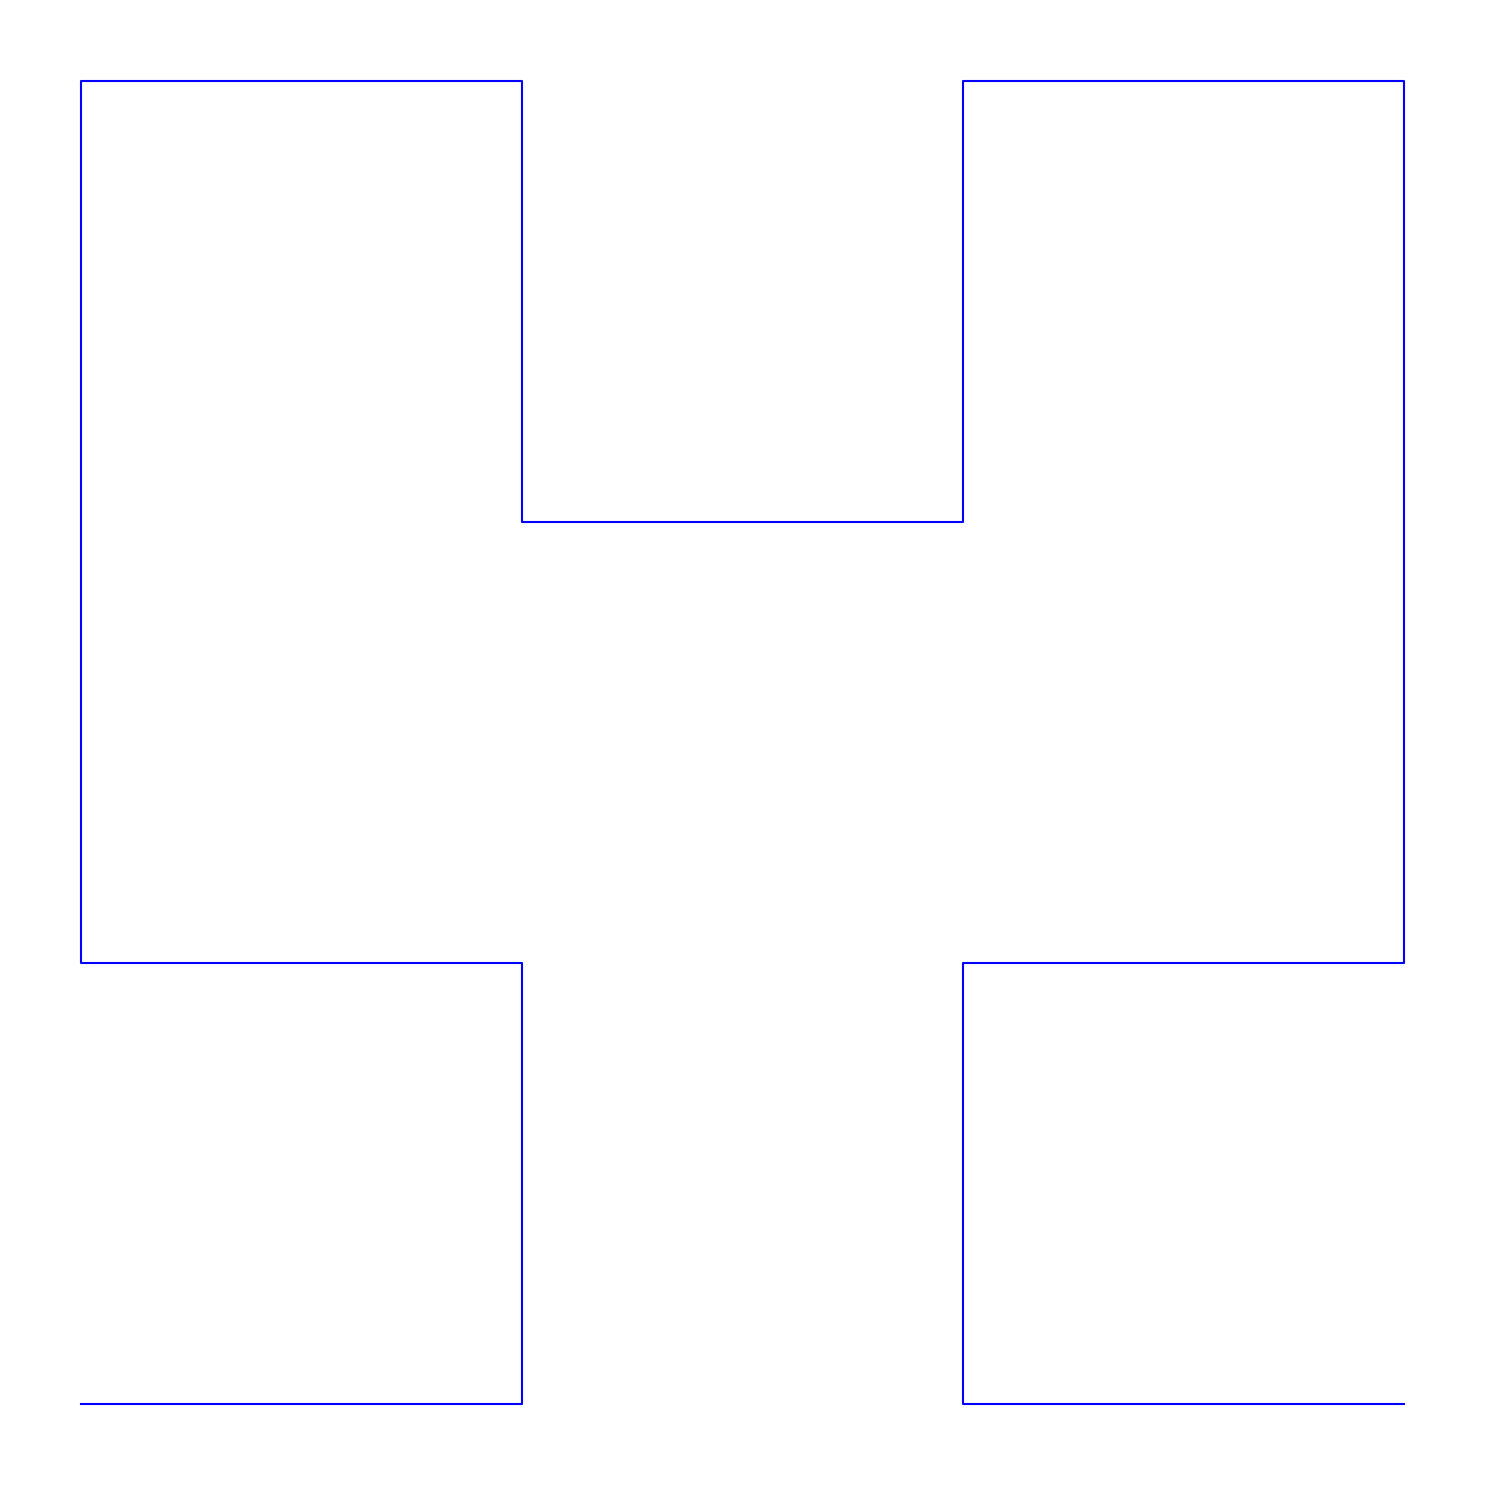
\includegraphics[width=\textwidth]{plots/hilbert_curve_level2.png}
        \caption{Кривая Гильберта 2-го порядка \\ Всего сегментов: 15}
    \end{subfigure}
    \\
    \begin{subfigure}{0.42\textwidth}
        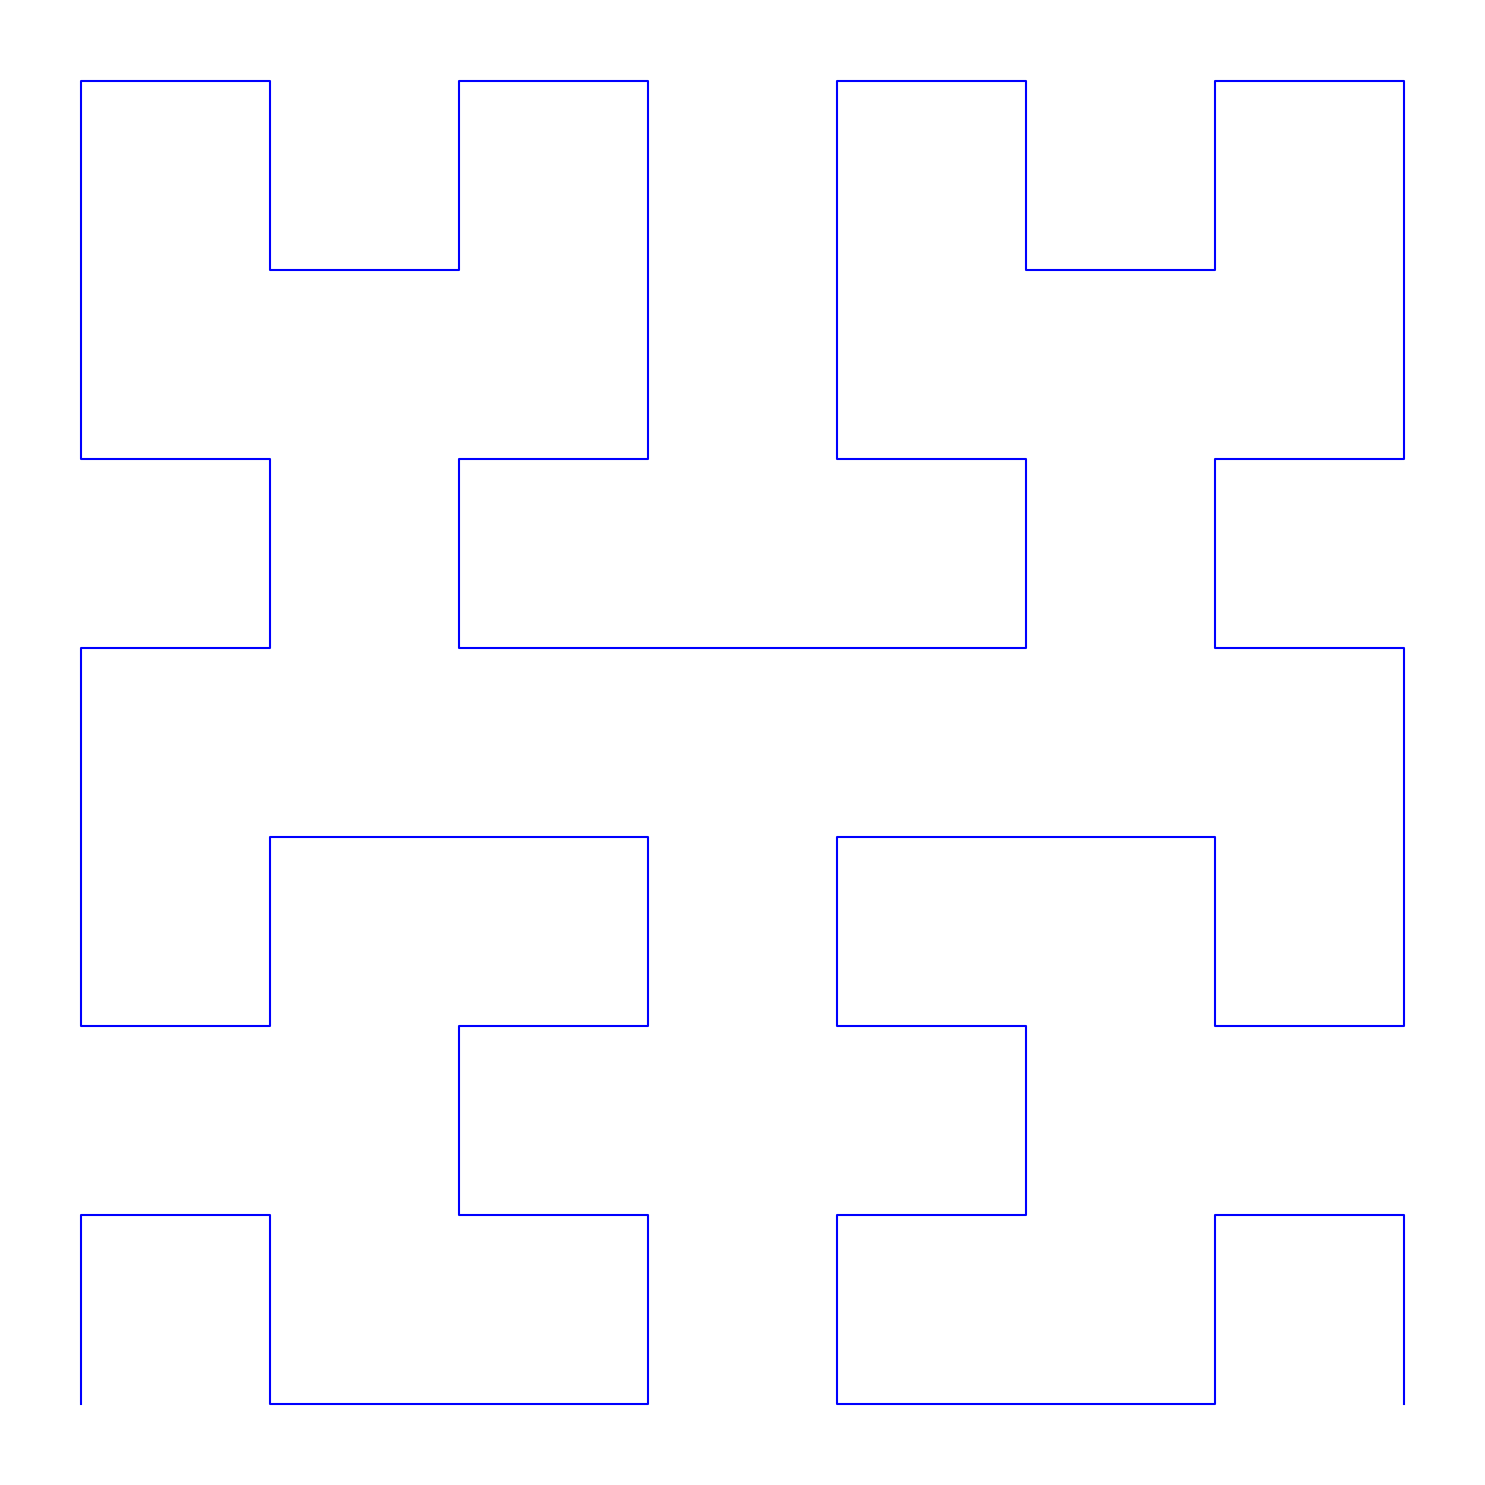
\includegraphics[width=\textwidth]{plots/hilbert_curve_level3.png}
        \caption{Кривая Гильберта 3-го порядка \\ Всего сегментов: 63}
    \end{subfigure}
    \hfill
    \begin{subfigure}{0.42\textwidth}
        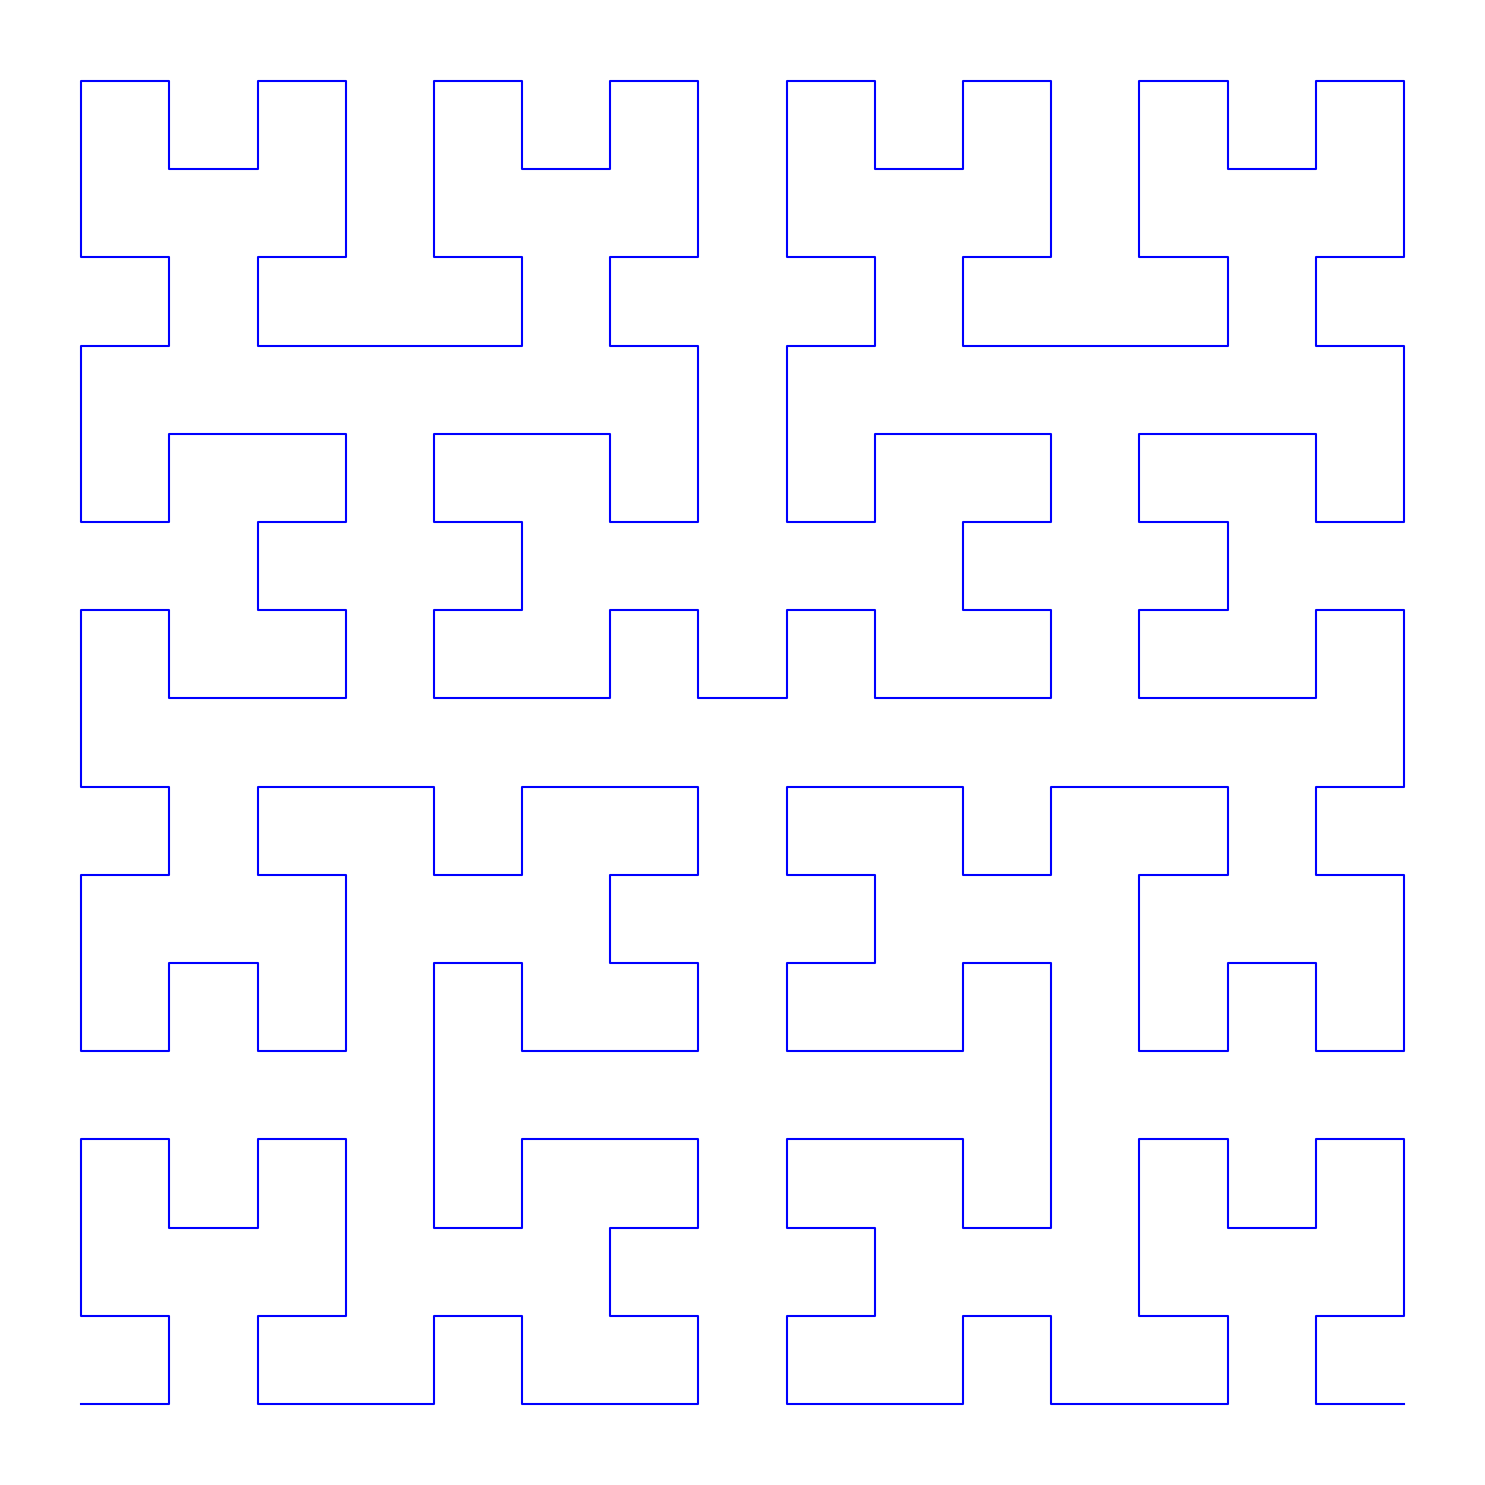
\includegraphics[width=\textwidth]{plots/hilbert_curve_level4.png}
        \caption{Кривая Гильберта 4-го порядка \\ Всего сегментов: 255}
    \end{subfigure}
    \\
    \begin{subfigure}{0.42\textwidth}
        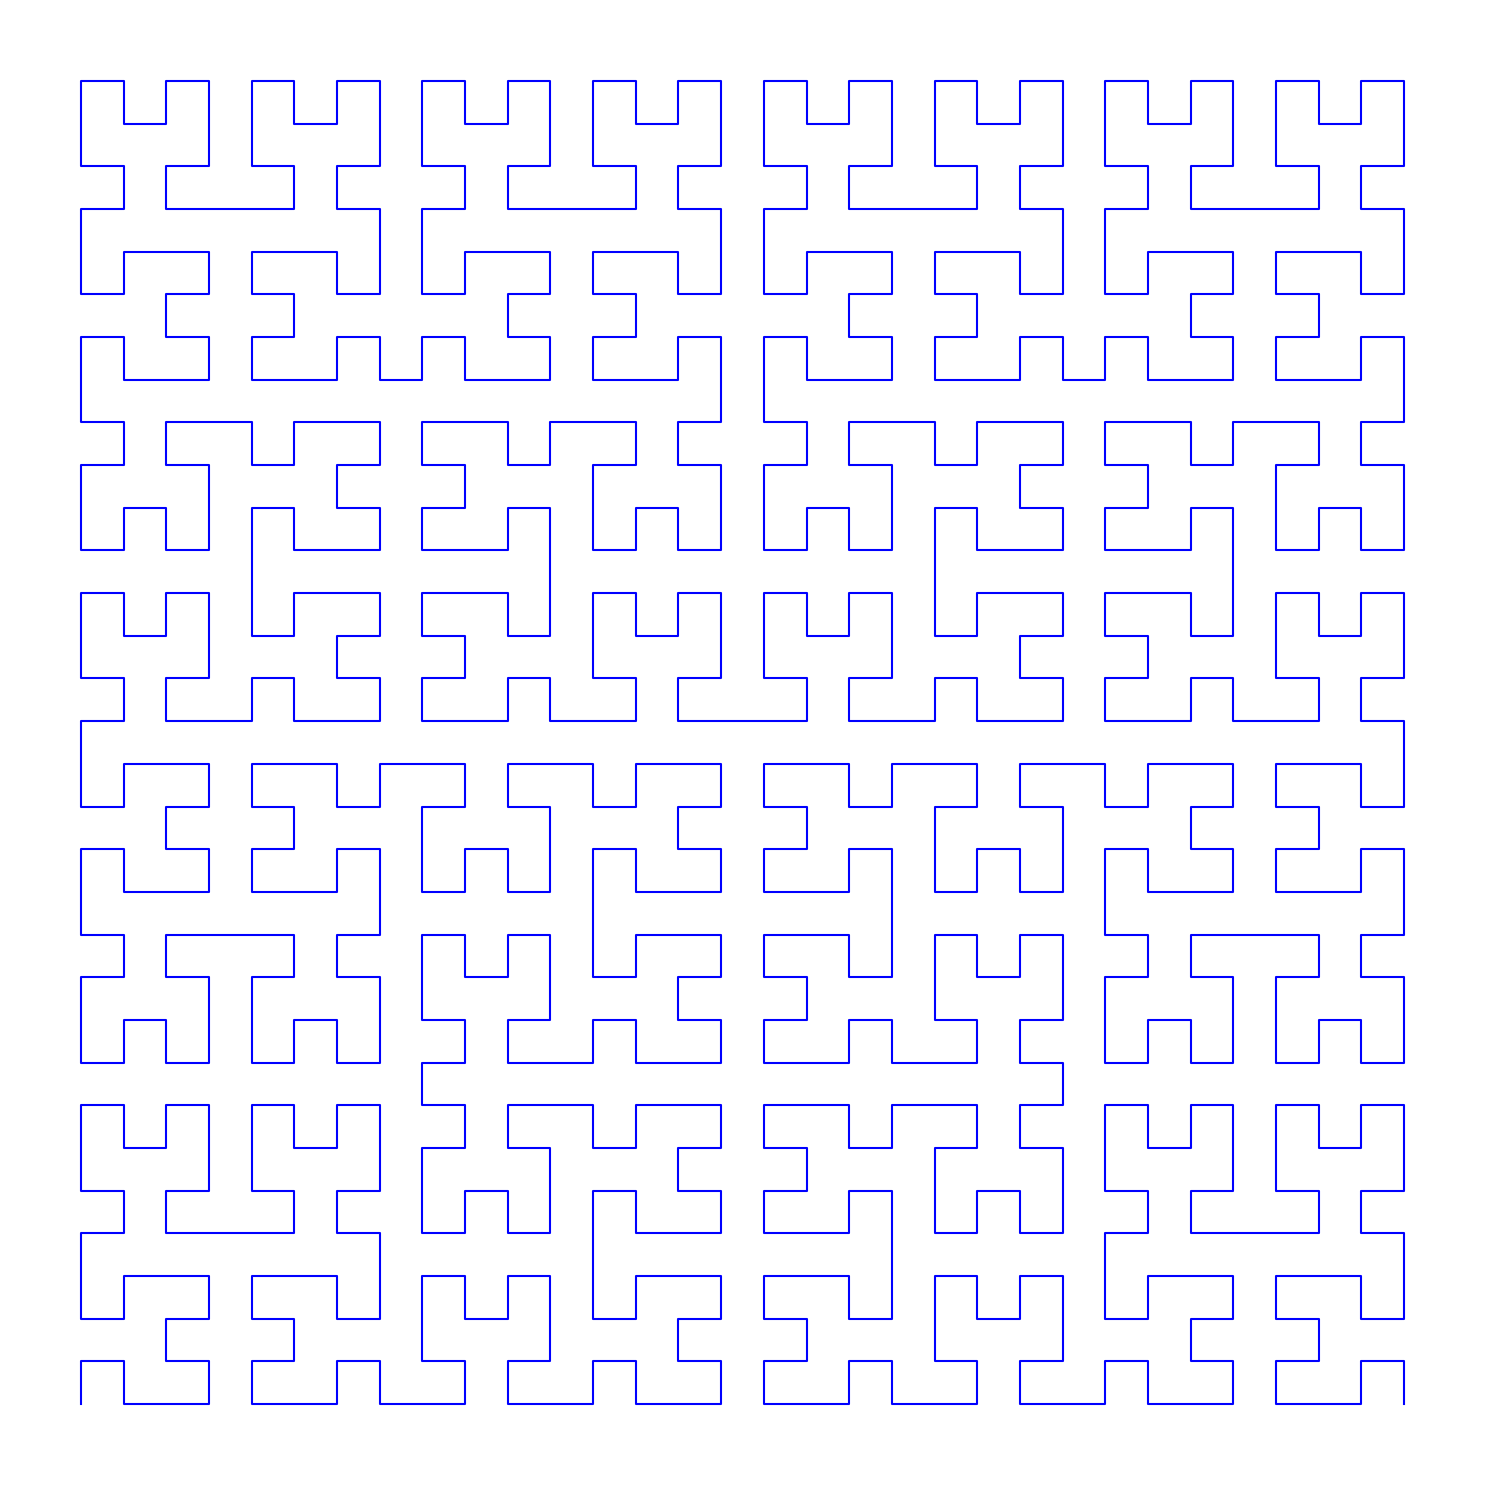
\includegraphics[width=\textwidth]{plots/hilbert_curve_level5.png}
        \caption{Кривая Гильберта 5-го порядка \\ Всего сегментов: 1,023}
    \end{subfigure}
    \hfill
    \begin{subfigure}{0.42\textwidth}
        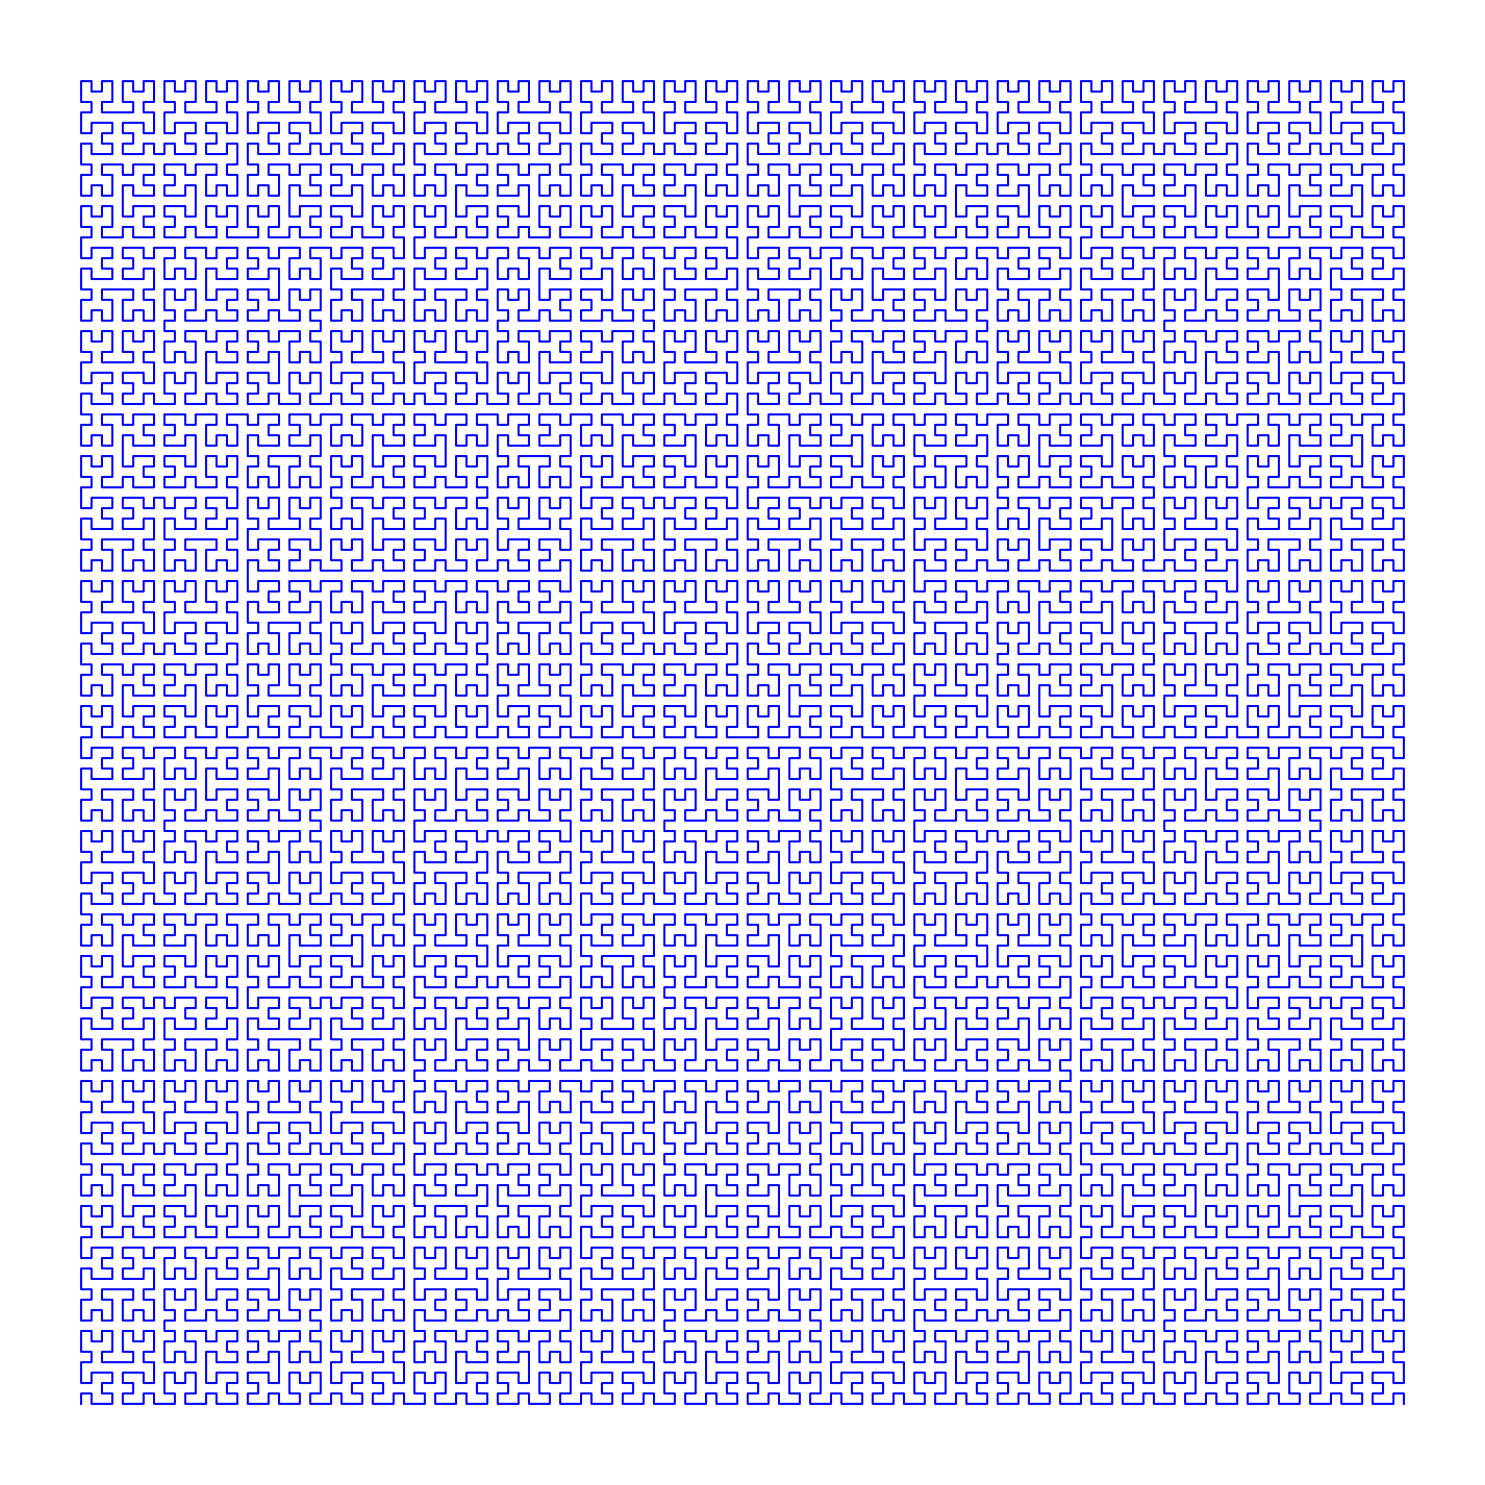
\includegraphics[width=\textwidth]{plots/hilbert_curve_level7.png}
        \caption{Кривая Гильберта 7-го порядка \\ Всего сегментов: 16,383}
    \end{subfigure}
    \caption{Построения кривой Гильберта разных порядков}
\end{figure}

\subsection{Анализ структуры}

Кривая Гильберта обладает рядом интересных свойств:
\begin{itemize}
    \item \textbf{Сюръективность.} Кривая Гильберта не позволяет биективно отобразить отрезок в квадрат, потому что \( p_n\colon [0,1]\twoheadrightarrow [0,1]^2 \) при \( n\to\infty \) имеет бесконечное число самопересечений. В частности, центральной точке соответствуют \( p(\frac{1}{6}) \), \( p(\frac{1}{2}) \) и \( p(\frac{5}{6}) \).\footnote{\href{https://thatsmaths.com/2022/08/11/space-filling-curves-part-ii-computing-the-limit-function/}{That's Maths: Space-Filling Curves, Part II}}
    \item \textbf{Недифференцируемость.} Несмотря на непрерывность отображения \( p \), оно нигде не дифференцируемо в силу более сильного утверждения для всюду плотных кривых.\footnote{\href{https://www.google.com/books/edition/Space_Filling_Curves/cP_ZBwAAQBAJ?hl=en&gbpv=1&pg=PA34&printsec=frontcover}{Sagan H. Space-Filling Curves. Springer-Verlag, 1994. Глава 3, стр. 34-36}}
    \item \textbf{Самоподобие.} Если увеличить любой подквадрат в \( 2n \) раз, мы получим кривую в точности похожую на всю кривую.
\end{itemize}

